\section{Modifications - \textit{DRAFT}}
\label{modifications}

This chapter is a review of the modifications made on the prototype to make a fully functional version of Virtual POP-C++ for the ViSaG project.

\subsection{Ability to compile two different versions of POP-C++}
As the Virtual version of POP-C++ is just installed on the admin-VM, the ability to compile a standard version (without virtual modifications) is a great choice for the end user. \s

To make this optional compilation possible, two objects have been created: 

\begin{itemize}
\item VirtualJobMgr: this object inherits from the JobMgr and overwrites the needed methods. 
\item VirtualPOPCSearchNode: this object inherits from the POPCSearchNode and overwrites the needed methods.
\end{itemize}

All the modifications related to the virtual version are now made in the VirtualJobMgr and in the VirtualPOPCSearchNode. A VirtualPOPCSecurityManager will certainly be needed. This modification will let the future version of POP-C++ evolve on the same basis and the merging needs will be less important. \s

\textbf{Files created:} ./lib/virtual\_jobmgr.ph, ./lib/virtual\_jobmgr.cc, ./lib/virtual\_popc\_search\_node.ph, ./lib/virtual\_popc\_search\_node.cc\s

\textbf{Files modified:} ./configure.ac, ./lib/jobmgr.ph, ./lib/jobmgr.cc, ./lib/popc\_search\_node.ph, ./script/popc\_setup.in\s

\textit{FULL EXPLANATION ...}

%
% HYPERVISOR INFORMATION
%

\subsection{Hypervisor information}
Instead of being stored in environment variable, the information relative to the hypervisor connection have been stored in the VirtualJobMgr configuration file. This file is located under \textit{POPC\_LOCATION}/etc/virtual.conf. The installation script is now writing the information directly into this configuration instead of writing them into a script that initialize the environment variables. \s

The JobMgr constructor retrieves all the information stored in the configuration file. These values are stored into attributes and used when needed.\s

\textbf{Files modified : } ./lib/virtual\_jobmgr.cc, ./lib/virtual\_jobmgr.ph, ./script/popc\_setup.in

\subsubsection{Hiding sensitive configuration information}
The virtual configuration file contains some sensitive information as hypervisor username and password and worker guest username and password. To avoid any bad usage of these information, this file must be encrypted. We have two options to encrypt this file. 

\begin{enumerate}
\item \textbf{Symmetric encryption}: using the same key to encrypt and decrypt the configuration file. \textit{TODO -- Figure}
\item \textbf{Asymmetric encryption}: using a private/public key pair. One key is used to encrypt the file and the second to decrypt it. \textit{TODO -- Figure} 
\end{enumerate}

In our case, we choose to use a symmetric encryption algorithm known as Rijndael or AES. The end of this section explain the steps to done in POP-C++ to encrypt the virtual configuration file. \s

The first step is to generate a key and encrypt the information about the virtual configuration. Figure \ref{fig:cipher1} shows this first step. During the compilation of POP-C++, a key is generated and integrated to the executable files. A small program is compiled to be able to encrypt the information about the virtual configuration given during the POP-C++ installation. This program is called \textbf{popcipher}. As shown in Figure \ref{fig:cipher1}, the JobMgr configuration file is not encrypted at all. Only the virtual configuration file is processed by \textbf{popcipher} as this file includes important passwords. 


\begin{figure}[ht]
	\caption{POP-C++ Virtual Configuration encryption (Step one)}
  	\centering
	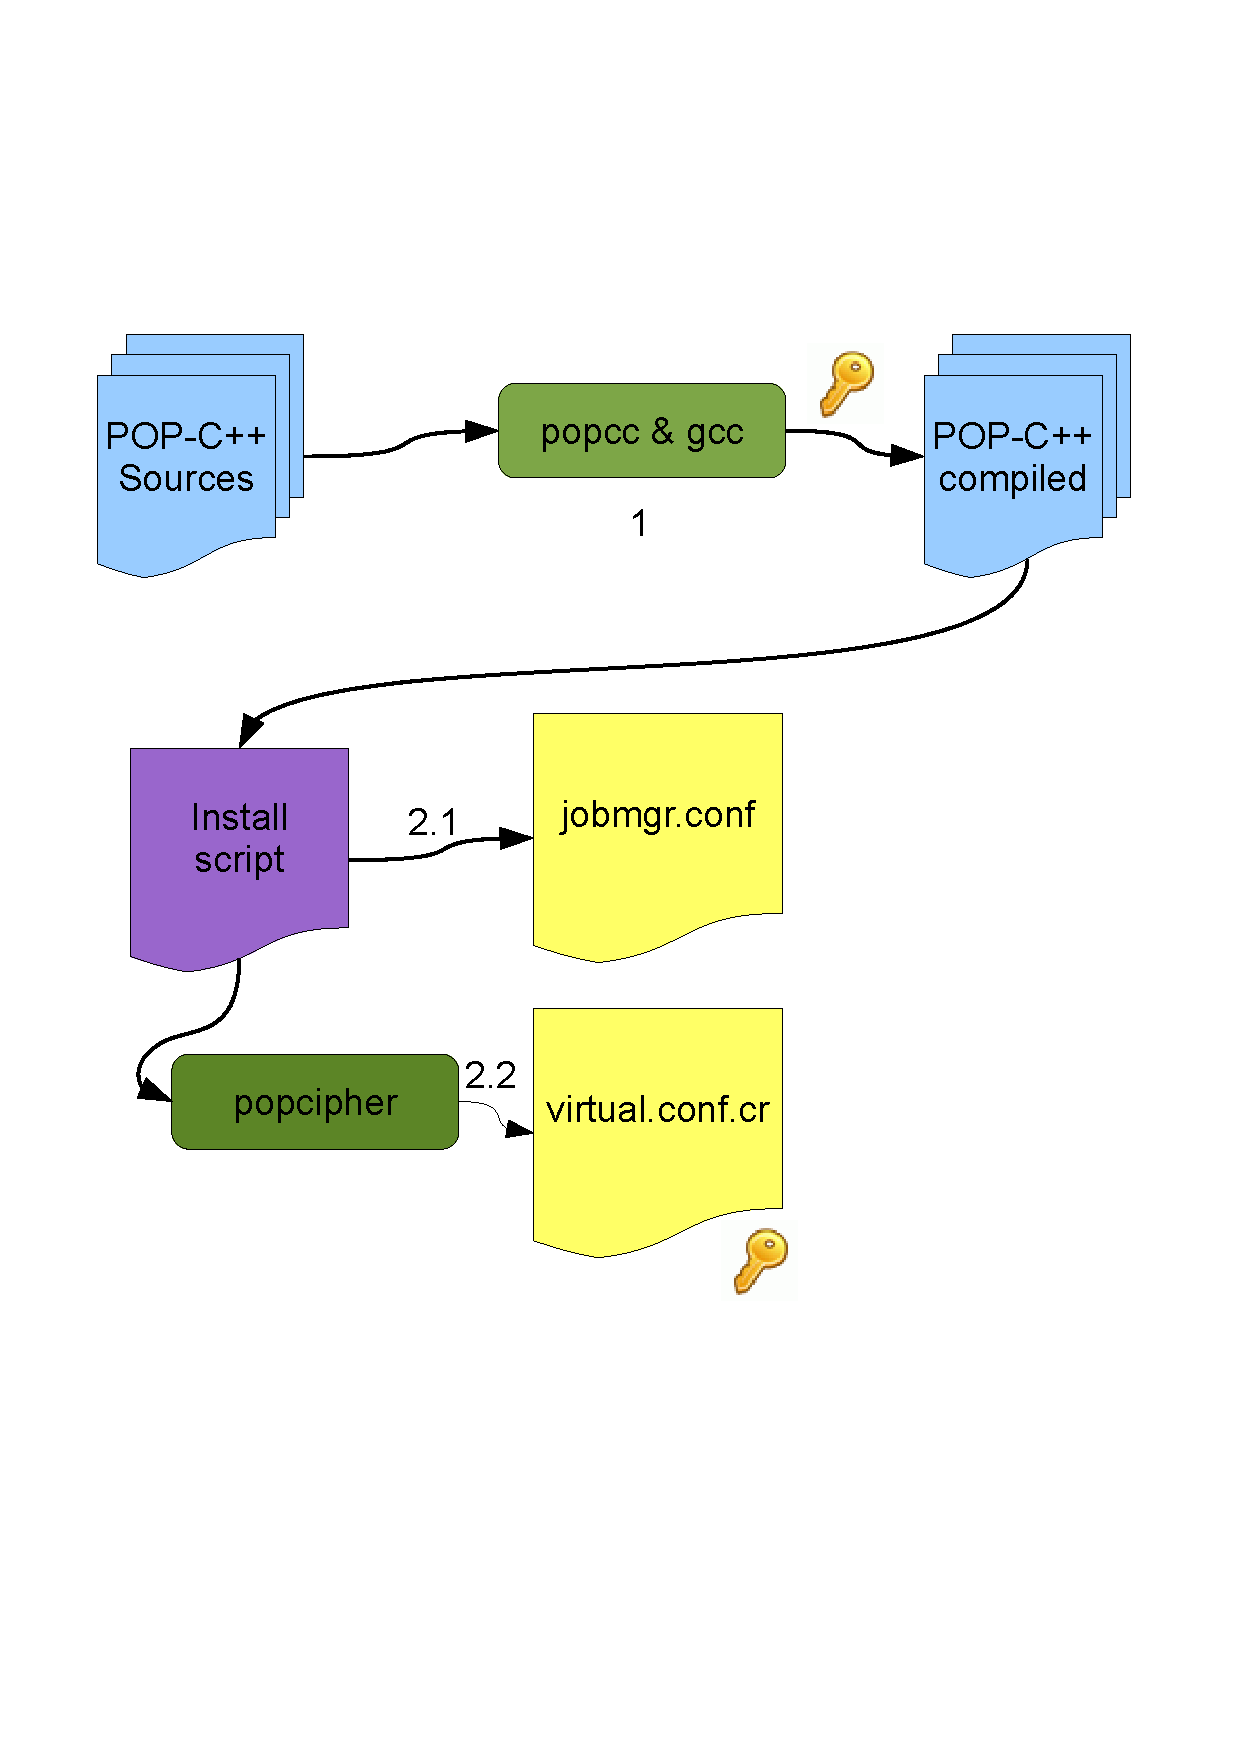
\includegraphics[width=0.5\textwidth]{./pic/cipher1.pdf}
	\label{fig:cipher1}
\end{figure}

Once the virtual configuration file is encrypted, POP-C++ need a way to read these information. Figure \ref{fig:cipher2}shows the starts of POP-C++ Global Services. Once the Virtual Secure JobMgre (VirtSecureJobMgr) is started by the "SXXpopc" script, this object will read the virtual.conf.cr file. This object has the ability to decrypt this file, as during the compilation of POP-C++, the generated key has been included in its executable. The VirtSecureJobMgr decrypts the virtual.conf.cr file and use its information directly in memory. All the information located in the jobmgr.conf file are read as usual as they are all in clear.

\begin{figure}[ht]
	\caption{POP-C++ Virtual Configuration decryption (Step two)}
  	\centering
	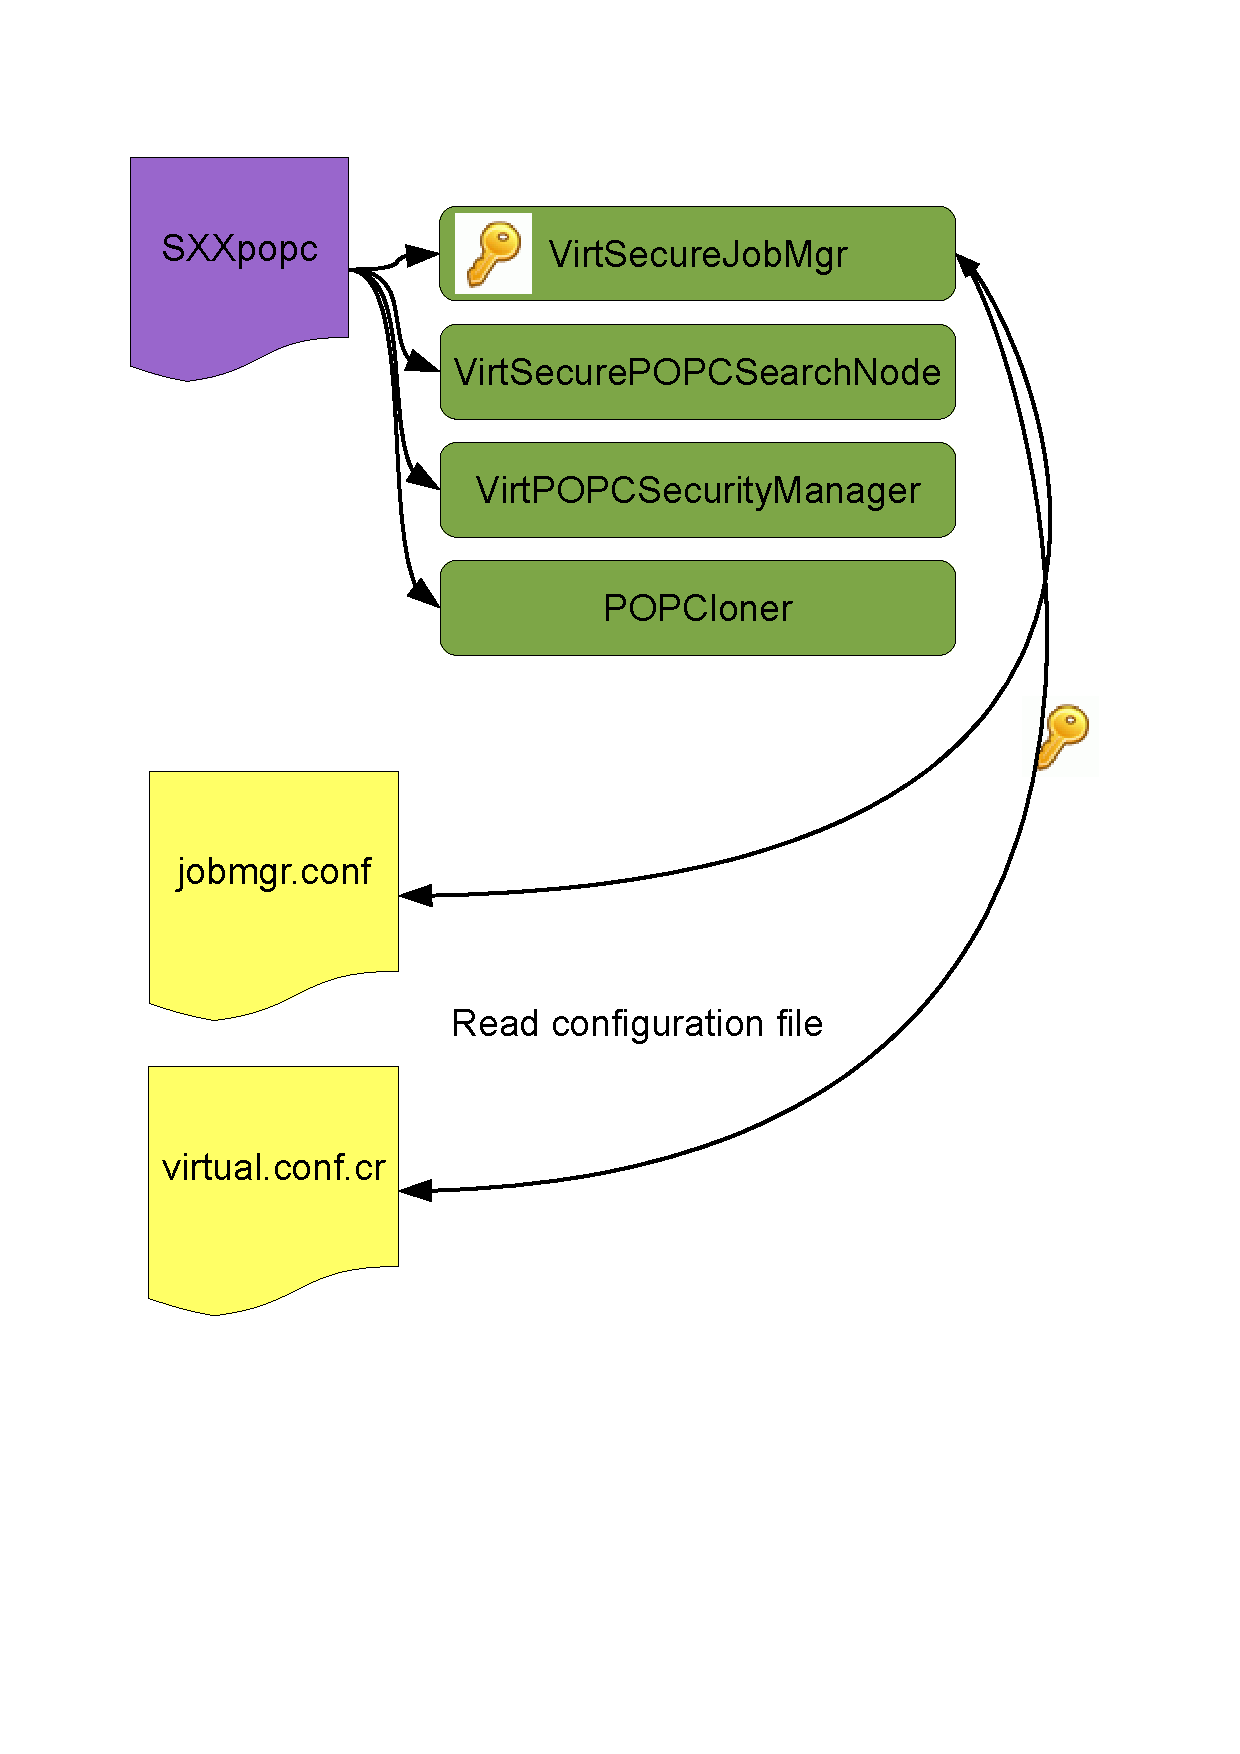
\includegraphics[width=0.5\textwidth]{./pic/cipher2.pdf}
	\label{fig:cipher2}
\end{figure}

%
% POP APPLICATION IDENTIFIER
%
\subsection{POP Application Identifier}
The AppCoreService has been modified to generate the POP Application ID. This ID is generated in the constructor of this object. The "Request" object has also been modified to include this ID. Just before launching the resource discovery, the JobMgr will contact the AppCoreService to know the POPAppID and set it in the request. The other JobMgrs contacted will know for which application a request has been launched. \s

For more information about the POP Application Identifier, please refer to the document "POP-C++ over SSH Tunnel"\cite{popcssh} in section 7.1.\s

In addition to these modifications, the reservation process must also include the POPAppID. The "struct Resources" have been modified to include the POPAppID. This struct is defined in the JobMgr header file. The "Reserve" method must now accept the POPAppId as a parameter. At this point, the JobMgr has all the information to manage the different VM worker.\s

\textbf{Files modified : } ./include/request.h, ./include/Makefile.am, ./lib/request.cc, ./lib/appservice.ph, ./lib/appservice.cc, ./lib/jobmgr.cc, ./lib/Makefile.am\s

\textbf{Files added : } ./include/popwayback.h, ./lib/popwayback.cc

%
% VIX COMPILATION
%
\subsection{POP-C++ and VIX compilation}
Some modifications have to be made to be able to compile POP-C++ with the VIX library. The modifications are listed below : \s

\textbf{File: configure.ac:}\\
As the VIX API does not install a ".pc" file for the pkg\_config function. We have to declare the \_CFLAGS and the \_LIBS marco for VIX. The lines below have been added to the "configure.ac" file. \s

\begin{lstlisting}
VIX_CFLAGS="-lvixAllProducts -ldl"
VIX_LIBS="-I/usr/include/vmware-vix"
AM_SUBST([VIX_CFLAGS])
AM_SUBST([VIX_LIBS])
\end{lstlisting}\s

\textbf{File: ./lib/Makefile.am:}\\
The input Makefile located in the "lib" directory must also be modified. The VIX macros must be added to the macro "AM\_CXXFLAGS". \s

\begin{lstlisting}
AM_CXXFLAGS= OTHER_FLAGS $(VIX_CFLAGS) $(VIX_LIBS)
\end{lstlisting}\s

With those modifications, POP-C++ can now be compiled with the VMware VIX API. \s

\textit{NOTE:} The VIX API must be installed on the machine which compile POP-C++ in its Virtual version. 


\subsection{Using VIX to get the worker VM IP address}
The VIX API allow us to read some properties on the guest VM. This ability is used to read the IP address of the guest VM. The process is going as follows:

\begin{enumerate}
\item Connect to the hypervisor (VixHost\_Connect())
\item Get a pointer to the VM (VixHost\_OpenVM())
\item Power on the VM (VixVM\_PowerOn())
\item Waiting for the VMware tools to be ready (VixVM\_WaitForToolsInGuest())
\item Read the variable "ip" (VixVM\_ReadVariable())
\end{enumerate}

\textit{NOTE:} For the full code, please see the file ./lib/ESXWrapper.cc method "\_popc\_domainGetIpAddress(POPvm \&vm)"

\subsection{Using VIX to send and write the admin VM public key on worker VM}
The VIX API has two very interesting function that allow us to send a file on the worker VM and to execute a command on the worker VM. We have to send the admin VM public key and write it in the authorized\_keys file on the worker VM. The process to do this using VIX is going as follows: \s

\begin{enumerate}
\item Connect to the hypervisor (VixHost\_Connect())
\item Get a pointer to the VM (VixHost\_OpenVM())
\item Power on the VM (VixVM\_PowerOn())
\item Waiting for the VMware tools to be ready (VixVM\_WaitForToolsInGuest())
\item Login in the guest VM (VixVM\_LoginInGuest())
\item Copy the admin public key file on the guest VM (VixVM\_CopyFileFromHostToGuest())
\item Execute a command on the guest to write the key (VixVM\_RunProgramInGuest())
\end{enumerate}

\textit{NOTE:} For the full code, please see the file ./lib/ESXWrapper.cc method "\_popc\_sendLocalPublicKey(POPvm \&vm)"

\subsection{Cloning function implementation}
As no built-in cloning function has been found either in the VIX API or in libvirt, this function has been implemented from scratch. The wrapper method "\_popc\_domainClone(POPvm \&original, POPvm \&clone)" does the whole process. As this process could take sometimes, this function will create a child process. 

\subsection{Requirements}
To be able to run the POP-C++ Virtual version, the following requirements must be fulfilled:





\begin{center}
\begin{tabular}{|p{1.8cm}|p{3.3cm}|p{2.7cm}|p{2.6cm}|p{1.5cm}|p{1.5cm}|}
\hline
\textbf{VM Type} & \textbf{POP-C++ version}	& \textbf{VMware tools} & \textbf{VMware CLI} & \textbf{VIX} & \textbf{libvirt}\\ \hline
Admin & Virtual Secure & X & >= 4.1 & >= 10.1 & >= 0.8.5\\ \hline
Worker & Secure & X & - & - &- \\ \hline

\end{tabular}
\end{center}\s

\begin{itemize}


\item VMware ESXi 4.1 or later must be installed as the hypervisor.
\item The VMware tools 8.3.2 build-257589 or later must be installed on the worker VM and on the Admin VM.
\item The VIX API 1.10 or later must be installed on the admin VM.
\item libvirt 0.8.3 or later must be installed on the admin VM.
\end{itemize} 


\section{Ability to manage more than one VM}
In the first prototype of VPOP-C++, the JobMgr was able to manage only one VM. In the final version, the JobMgr must be able to manage many VM. To enable this ability, some change have been made in the Wrapper interface. The wrapper interface was designed for one VM only. A new object called "POPvm" is now holding all the information about a specific VM. This object is passed through the Wrapper. Additional information can be inserted in the "POPvm" object without modifying the "Wrapper" (could be done for different virtualization platform than ESXi). 